\chapter[Resultados]{Resultados}

\section{Implementação dos \textit{Shaders}}

	Primeiramente foi feita a implementação dos \textit{shaders} para plataforma \textit{Android} utilizando o paradigma de orientação a objetos, em que o diagrama de classes (Figura \ref{class_diagram}) mostra como ele está estruturado. Ele mostra um conjunto de classes e seus relacionamentos, sendo o diagrama central da modelagem orientada a objetos. 

	\begin{figure}[h]
	\centering
		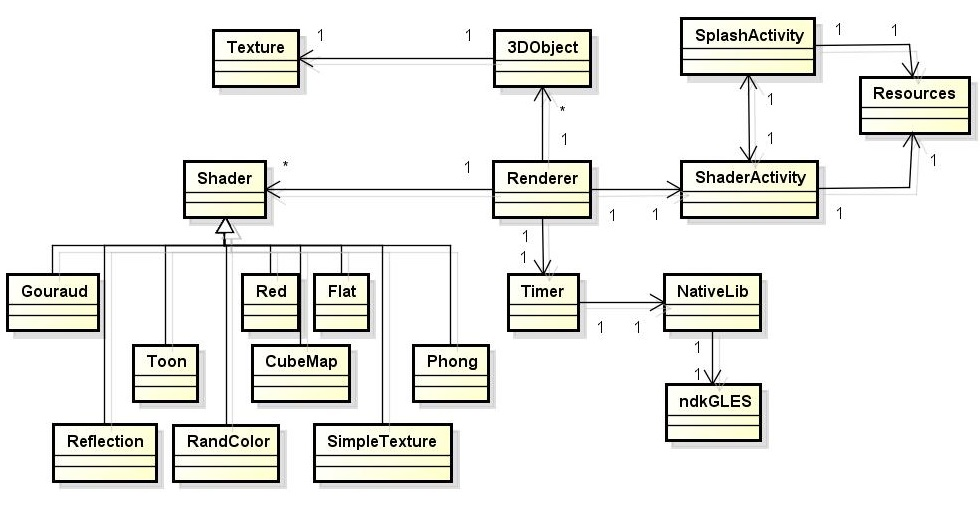
\includegraphics[keepaspectratio=true,scale=0.6]{figuras/class_diagram.jpg}
	\caption{Diagrama de Classe da Implementação em \textit{Android}}
	\label{class_diagram}
	\end{figure}

	\subsection{Classes \textit{Shader Activity} e \textit{Splash Activity}}

	\begin{figure}[h]
	\centering
		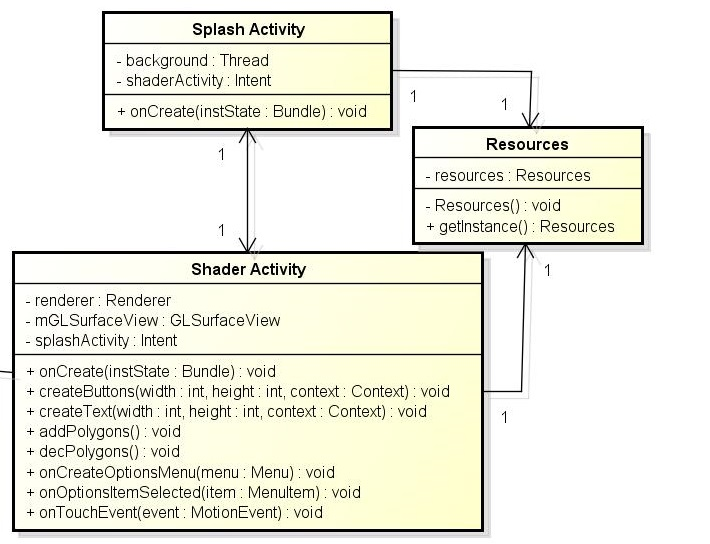
\includegraphics[keepaspectratio=true,scale=0.6]{figuras/shader_splash.jpg}
	\caption{Detalhamento das classes \textit{Shader Activity}, \textit{Splash Activity} e \textit{Resources}}
	\label{shader_splash}
	\end{figure}

	De acordo com \ref{androidsdkmanager}, a plataforma \textit{Android} utiliza o termo \textit{Activity} para descrever a tela de \textit{front-end} da aplicação que interage com o usuário. Ela possui elementos de \textit{design} como texto, botões, gráficos, entre outros. No contexto deste trabalho, há duas classes \textit{Activity}, a \textit{Shader} e a \textit{Splash}. 

	A \textit{Splash Activity} (Figura  \ref{splash_act}) é responsável pela visualização da tela de \textit{loading} enquanto carrega os recursos necessários para o programa (como a leitura dos modelos tridimensionais em formato obj e das imagens usadas para texturização) por meio do uso de \textit{thread}. Estes recursos são setados por meio da classe chamada \textit{Resources}, que utiliza o padrão de projeto chamado \textit{Singleton}, que garante a existencia de apenas uma instância da classe, que será acessada posteriormente.

	\begin{figure}[h]
	\centering
		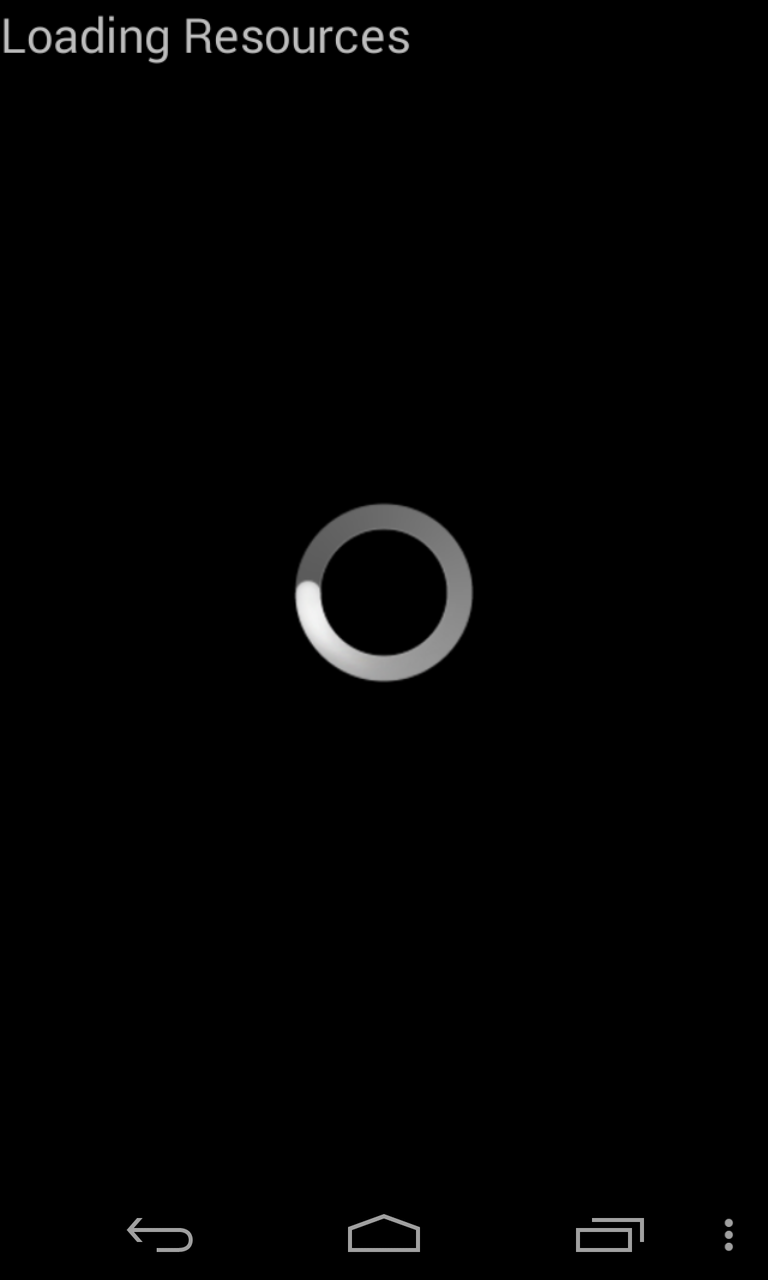
\includegraphics[keepaspectratio=true,scale=0.2]{figuras/splash_act.png}
	\caption{Tela da \textit{Splash Activity}}
	\label{splash_act}
	\end{figure}

	A \textit{Shader Activity} (Figura  \ref{shader_act}) é responsável pela  instanciação da classe \textit{Renderer}, que renderiza os gráficos tridimensionais utilizando a biblioteca \textit{OpenGL ES}. Além disso, ela controla os eventos de \textit{touch}, que permitem escalar e mover o objeto, além de disponibilizar os menus que trocam de \textit{shaders}, os botões que aumentam, diminuem o número de polígonos, a informação do tempo de renderização e a de quantidade de polígonos. Aumenta-se o número de polígonos por meio da troca de objetos que possuem arquivos obj diferentes, que já foram carregados pela \textit{Splash Activity}. 

	\begin{figure}[h]
	\centering
		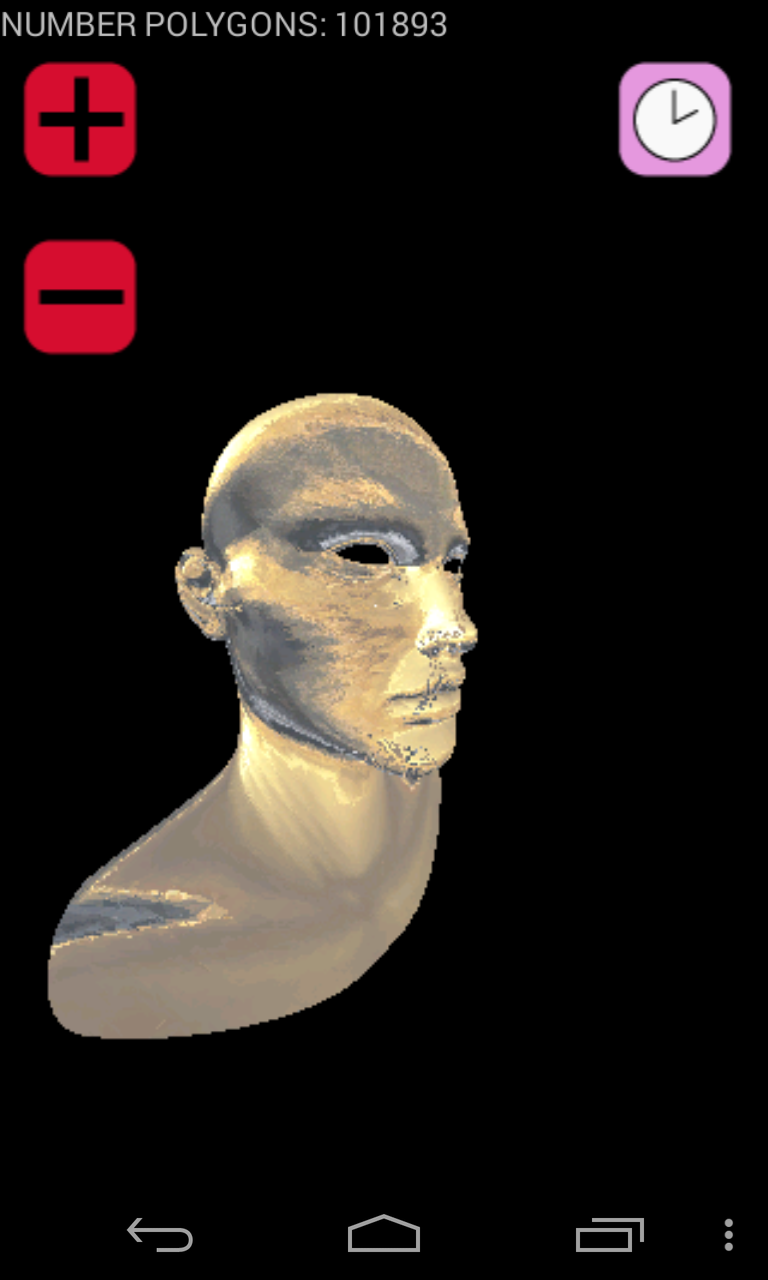
\includegraphics[keepaspectratio=true,scale=0.2]{figuras/shader_act.png}
	\caption{Tela da \textit{Shader Activity}}
	\label{shader_act}
	\end{figure}

	Devido à limitação de memória do dispositivo móvel e os vários objetos com diferentes números de polígonos, não é possível carregar todos de uma só vez. Assim, foi necessário dividir esta quantidade objetos por vez, em que quando chega-se ao último objeto (tanto adicionando, quanto decrementando), volta-se novamente para a \textit{Splash Activity}, a fim de carregar os novos objetos e ir novamente para a \textit{Shader Activity}, a fim de renderizá-los.

	\subsection{ Classes \textit{3DObject} e \textit{Texture}}   

	\begin{figure}[h]
	\centering
		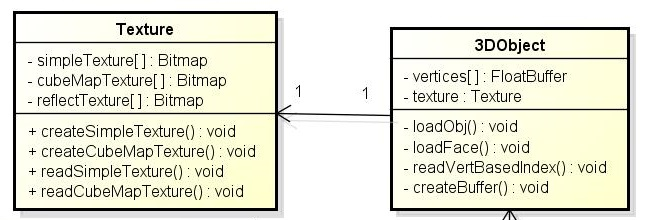
\includegraphics[keepaspectratio=true,scale=0.6]{figuras/object_texture.jpg}
	\caption{Detalhamento das classes \textit{3DObject} e \textit{Texture}}
	\label{object_texture}
	\end{figure}

	A classe \textit{3DObject}, mostrada na Figura \ref{object_texture}, é responsável por ler o arquivo obj e armazenar, em um \textit{buffer}, os vértices de posição, normal e textura na ordem em que será renderizado. No \textit{buffer} cada coordenada relacionada a um vértice (posição, normal e textura) é armazenada alternadamente, como mostra a Figura \ref{buffer}.

	A classe \textit{Texture} cria as texturas utilizadas pelos \textit{shaders} \textit{SimpleTexture}, \textit{CubeMap} e \textit{Reflection}. Para gerar uma textura simples, primeiramente gera-se um objeto de textura \texttt{glGenTextures}, depois vincula-se a a textura a este objeto utilizando a função \texttt{glBindTexture} e carrega-se a imagem por meio da função \texttt{texImage2D}.  Para as texturas do \textit{CubeMap} e \textit{Reflection}, faz-se a mesma coisa, exceto que a função \textit{texImage2D} é feita seis vezes, em que cada textura representa uma face de um cubo. 

	\begin{figure}[h]
	\centering
		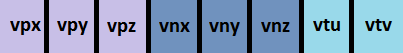
\includegraphics[keepaspectratio=true,scale=1.0]{figuras/buffer.png}
	\caption{Ordem das coordenadas de posição, normal e textura para um vértice}
	\label{buffer}
	\end{figure}

	\subsection{Classes \textit{Timer} e \textit{NativeLib}}      

	\begin{figure}[h]
	\centering
		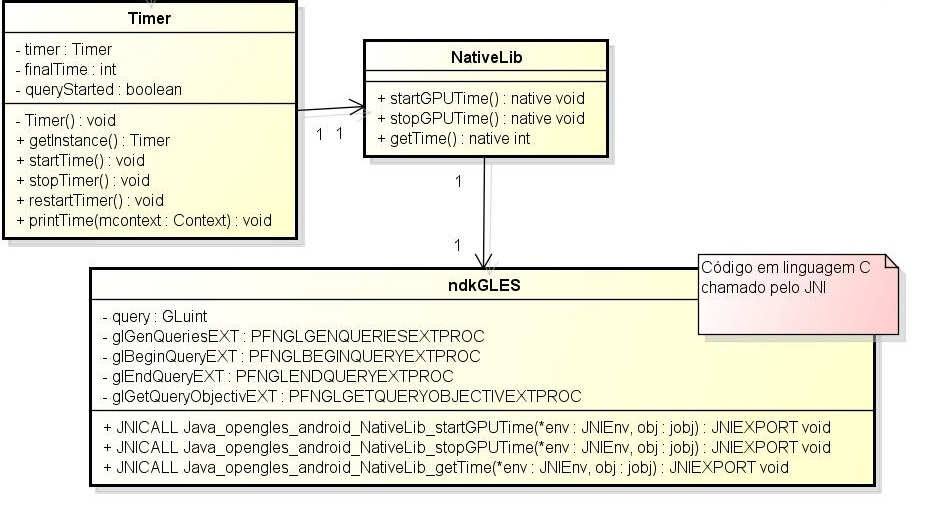
\includegraphics[keepaspectratio=true,scale=0.6]{figuras/timer_nativelib.jpg}
	\caption{Detalhamento das classes \textit{Timer} e \textit{NativeLib}}
	\label{timer_nativelib}
	\end{figure}

	A Figura \ref{timer_nativelib} detalha a classe \textit{Timer}, que realiza a média de dez medições do tempo (em nanosegundos) para cada objeto tridimensional, utilizando um \textit{shader} específico. Cada medição é feita utilizando a linguagem C e a extensão de \textit{OpenGL ES} chamada GL\_EXT\_disjoint\_timer\_query citada na Seção \ref{gpu}.  A integração entre o codigo em linguagem C e o código em Java é feita por meio da classe \textit{NativeLib}.

	\subsection{Classe \textit{Renderer}}    

	\begin{figure}[h]
	\centering
		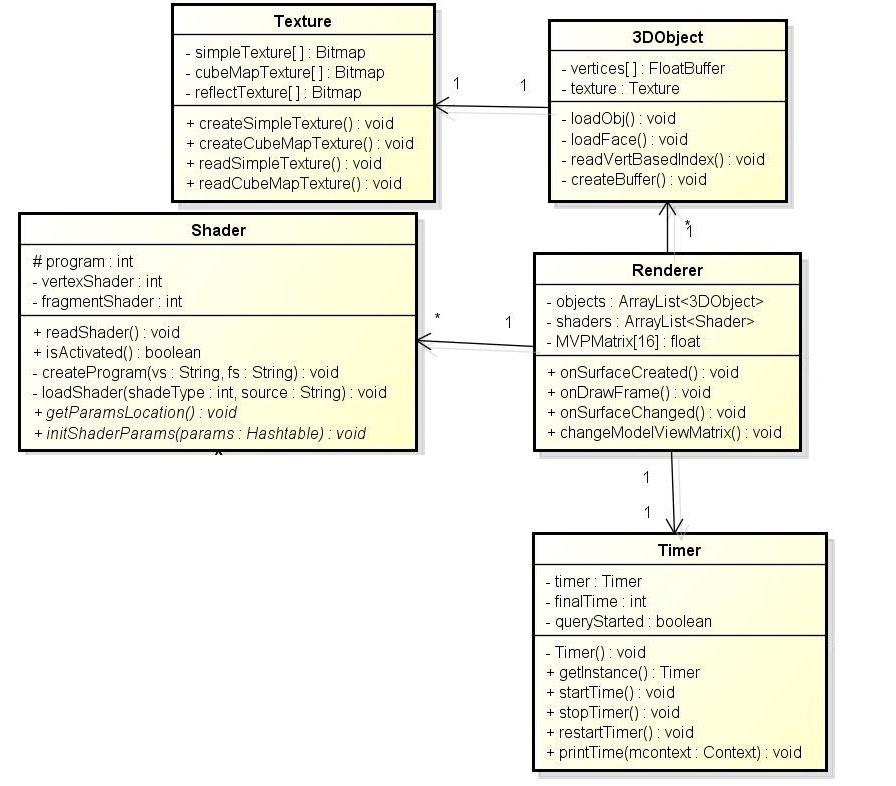
\includegraphics[keepaspectratio=true,scale=0.6]{figuras/renderer.jpg}
	\caption{Detalhamento da classe \textit{Renderer}}
	\label{renderer}
	\end{figure}

	A classe \textit{Renderer} (Figura \ref{renderer}) funciona como uma controladora, sendo o ponto principal  das chamadas provenientes da \textit{view} (\textit{ShaderActivity}) para a camada mais abaixo (\textit{3DObject}, \textit{Shader} e \textit{Timer}). Ela que implementa as funções da biblioteca \textit{OpenGL ES} \texttt{onSurfaceCreated},  \texttt{onDrawFrame} e \texttt{onSurfaceChanged}. A primeira função é chamada apenas uma vez quando a \textit{view} da \textit{OpenGL ES} é instanciada, em que faz-se todas as configurações nesta função, como por exemplo, criação de texturas. A segunda função é chamada em \textit{loop}, em que faz-se a renderização por meio da função \texttt{glDrawArrays}. 

	\subsection{Classe \textit{Shader}}      

	\begin{figure}[h]
	\centering
		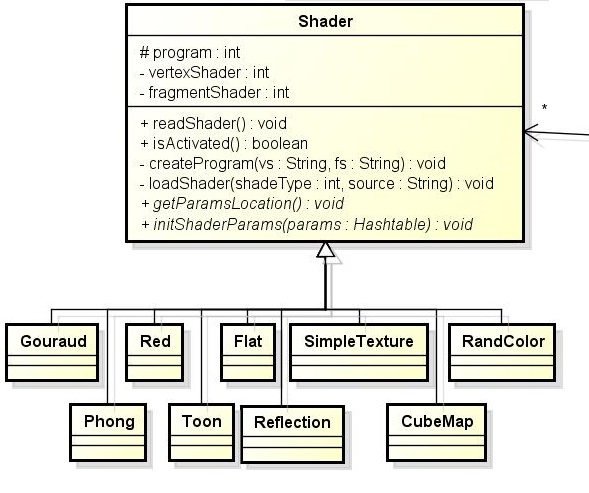
\includegraphics[keepaspectratio=true,scale=0.6]{figuras/shaders_diag.jpg}
	\caption{Detalhamento da classe \textit{Shader}}
	\label{shaders_diag}
	\end{figure}

	A classe \textit{Shader} (Figura \ref{shaders_diag}) é responsável por ler, fazer o \textit{attach} e o \textit{link} do \textit{ vertex} e do \textit{fragment shaders}. Além disso, ela possui os métodos abstratos \texttt{getParamsLocation} e \texttt{initShaderParams(Hastable params)}. Assim, todos os \textit{shaders} que herdam desta classe, são obrigados a implementar estes métodos. O primeiro método faz o armazenamento da localização de cada variável especificada dentro do \textit{shader}, já o segundo método inicializa estas variáveis por meio de um \textit{hash} que é passado como um parâmetro pela classe \textit{Renderer}.     

	\subsection{ \textit{Shaders} Implementados}    

	A fim de de poder fazer a análise da complexidade algorítmica, alguns \textit{shaders} foram implementados, em que cada um deles herdam da classe \textit{Shader} e implementam seus métodos abstratos. Estes \textit{shaders} podem ser vistos na Figura \ref{shaders_impl}.  

	\begin{figure}[h]
	\centering
		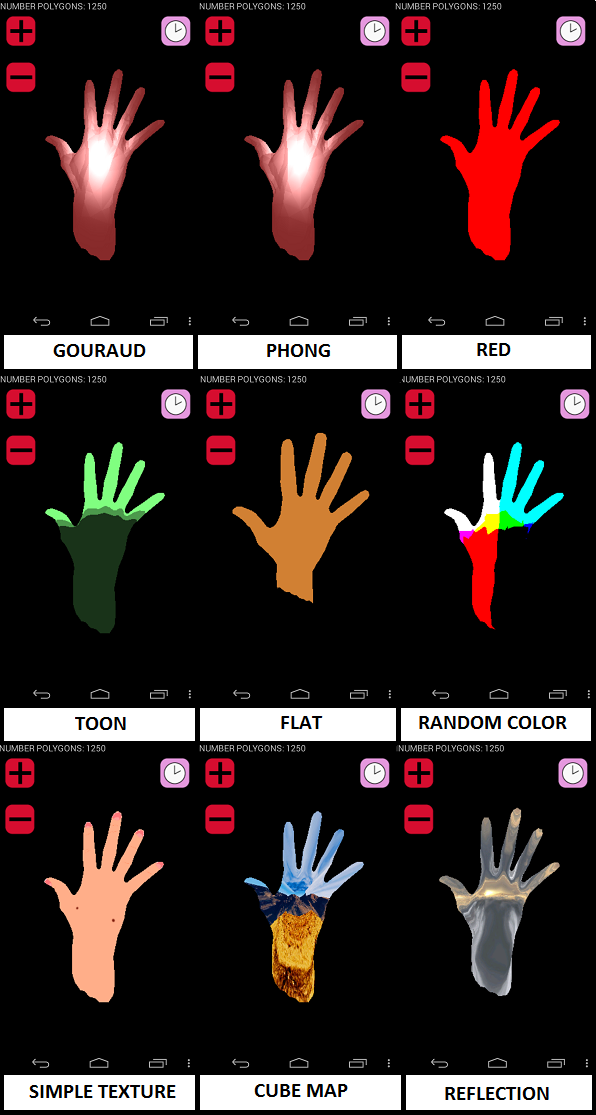
\includegraphics[keepaspectratio=true,scale=0.7]{figuras/shaders_impl.png}
	\caption{\textit{Shaders} Implementados}
	\label{shaders_impl}
	\end{figure}

	A seguir, alguns dos \textit{shaders} implementados serão explicados:

	\begin{itemize}
  	\item \textit{Phong Shader}
	\end{itemize}

	O \textit{vertex} e \textit{fragment shaders} do \textit{phong shading} implementam a técnica descrita na Seção \ref{flatgouphon}, em que primeiramente interpolam-se os valores das normais das primitivas e então computam-se os cálculos de luz para cada fragmento, utilizando as normais interpoladas. O Código \ref{codphongvs} e o Código \ref{codphongfs} mostram as definições do \textit{vertex} e \textit{fragment shaders}, respectivamente, em que para isso é necessário definir as propriedades do material pelo programa.  

	\lstinputlisting[language=C, label = {codphongvs}, caption = {\textit{Phong Shader}:  \textit{vertex shader}}]{codigos/phong_vs.txt}

	\lstinputlisting[language=C, caption =  {\textit{Phong Shader}:  \textit{fragment shader}}, label = {codphongfs}  ]{codigos/phong_ps.txt}
	

	\begin{itemize}
  	\item \textit{Red Shader}
	\end{itemize}

	
	O \textit{shader} que define a cor para vermelha é muito simples,  seu \textit{vertex shader} apenas estabelece que a posição do vértice  se dá pelo pela multiplicação da coordenada ( variável \texttt{aPosition} ) com a matriz de projeção, visualização e modelagem como é mostrada no Código \ref{codredvs}. 
	
	\lstinputlisting[language=C, caption = {\textit{Red Shader}:  \textit{vertex shader}}, label = {codredvs}]{codigos/red_vs.txt}

	Já o seu \textit{fragment shader} (Código \ref{codredfs}) estabele que todo fragmento possui a cor vermelha, por meio da palavra restrita \texttt{gl\_FragColor}.
	
	\lstinputlisting[language=C, caption = {\textit{Red Shader}:  \textit{fragment shader}}, label = {codredfs}]{codigos/red_ps.txt}

	\begin{itemize}
  	\item \textit{Toon Shader}
	\end{itemize}

	O  \textit{toon shader} calcula a intensidade da luz por vértice para escolher uma das cores pré-definidas, como é explicado na Seção ADICIONAR SEÇÃO. O Código  \ref{codtoonvs} mostra o cálculo da intensidade da luz por vértice, pegando primeiro a direção da luz (definida como uma variável \texttt{uniform} passada pelo programa) para depois fazer o produto escalar entre ela e a normal (cálculo da intensidade da luz).  

	\lstinputlisting[language=C,label = {codtoonvs}, caption = {\textit{Toon Shader}:  \textit{vertex shader}} ]{codigos/toon_vs.txt}

	A variável \textit{intensity} do tipo \textit{varying} é passada do \textit{vertex shader} para o \textit{fragment shader}, a fim de determinar qual das três cores será escolhida (Código \ref{codtoonfs}). 
  
 	\lstinputlisting[language=C, caption = {\textit{Toon Shader}:  \textit{fragment shader}}, label = {codtoonfs} ]{codigos/toon_ps.txt}

	\begin{itemize}
  	\item \textit{Simple Texture Shader}
	\end{itemize}

	O \textit{vertex shader} do \textit{simple texture shading} primeiramente armazena as coordenadas de textura numa variável do tipo \textit{varying} (Código \ref{codtexvs}), e as repassa para o \textit{fragment shader}, além de também definir a posição.  

	\lstinputlisting[language=C, caption =  {\textit{Simple Texture Shader}:  \textit{vertex shader}}, label = {codtexvs} ]{codigos/simple_tex_vs.txt}

	No Código \ref{codtexfs}, o \textit{fragment shader} por sua vez, utiliza a textura passada pelo programa e aplica a coordenada de textura, repassada pelo \textit{vertex shader}, no fragmento por meio da função  \texttt{texture2D}.

	\lstinputlisting[language=C, caption =  {\textit{Simple Texture Shader}:  \textit{fragment shader}}, label = {codtexfs} ]{codigos/simple_tex_ps.txt}

	\begin{itemize}	
  	\item \textit{CubeMap Shader}
	\end{itemize}

	 O \textit{CubeMap Shader} implementa a técnica descrita na Seção ADICIONAR SEÇÃO. O seu  \textit{vertex shader} é simples e só define a posição do vértice (Código \ref{codcubemapvs}). 

	\lstinputlisting[language=C, caption =  {\textit{CubeMap Shader}:  \textit{vertex shader}}, label = {codcubemapvs} ]{codigos/cubemap_vs.txt}

	O  \textit{fragment shader} (Código \ref{codcubemapps}), por sua vez, utiliza a função \texttt{textureCube} utiliza a normal para fazer o mapeamento da textura. 

	\lstinputlisting[language=C, caption =  {\textit{CubeMap Shader}:  \textit{fragment shader}}, label = {codcubemapps} ]{codigos/cubemap_ps.txt}
	
	\begin{itemize}
  	\item \textit{Reflection Shader}
	\end{itemize}

	O \textit{vertex shader} do \textit{shader} de reflexão é responsável por indicar que a posição do vértice se dá pela multiplicação da coordenada obtida pela variável \texttt{vec4 aPosition} com a matriz de projeção, visualização e modelagem, como é mostrado no Código \ref{codreflvs}. Além disso, ele declara dois vetores do tipo \textit{varying} (para passar ao \textit{fragment shader}) que estão relacionados com o vetor de direção da câmera e a normal. 

	\lstinputlisting[language=C, caption = {\textit{Reflection Shader}:  \textit{vertex shader}}, label = {codreflvs}]{codigos/reflection_vs.txt}

	No \textit{fragment shader}, a normal e o vetor de direção da câmera são utilizados para encontrar o vetor da direção da reflexão através da utilização da função \texttt{reflect}. Para corrigir a direção da normal, ela é multiplicada pela transposta da inversa da matriz de projeção, modelagem e visualização, como foi explicado na seção ADICIONAR LINK PARA SEÇÃO. O vetor da direção da reflexão é utilizado na função \textit{texteruCube} (Código \ref{codreflfs}), em que determina-se a cor do fragmento, baseando-se nesta direção e em uma imagem. 

	\lstinputlisting[language=C, caption = {\textit{Reflection Shader}:  \textit{fragment shader}}, label = {codreflfs}]{codigos/reflection_ps.txt}

\section{Plotagem e Aplicação do Método dos Mínimos Quadrados}

	Para a plotagem e aplicação do método dos mínimos quadrados, foi feito um programa em linguagem \textit{Python}, a fim de automatizar este processo. Ele é executado por linha de comando, em que passa-se como parâmetro o \textit{shader} desejado (Figura \ref{linhacomando}).

	\begin{figure}[h]
	\centering
		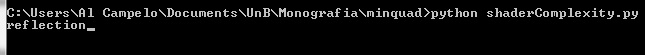
\includegraphics[keepaspectratio=true,scale=1.0]{figuras/linhacomando.jpg}
	\caption{Diagrama de Classes do código de automatização}
	\label{linhacomando}
	\end{figure}

	O programa encontra-se estruturado de acordo com a Figura \ref{minquad_diag}, em que a classe \textit{ReadCSV} é responsável por ler os arquivos CSV e fazer a média das métricas tanto para o \textit{vertex shader} como para o \textit{fragment shader}. Já a classe \textit{PlotChart}, faz a plotagem do gráfico do número de instruções por segundo por vértice \textit{versus} o número de polígonos e do gráfico do número de instruções por segundo por fragmento \textit{versus} o número de polígonos. Além disso, ele também plota o gráfico original juntamente com o gráfico após a aplicação do método dos mínimos quadrados. Por fim, o módulo \textit{LeastSquares} realiza o ajuste dos mínimos quadrados para uma reta e para polinômios de segundo e terceiro graus como explicado na Seção \ref{metminqua}. Ele também calcula os erros associados a cada ajuste e indica qual o menor. 

	\begin{figure}[h]
	\centering
		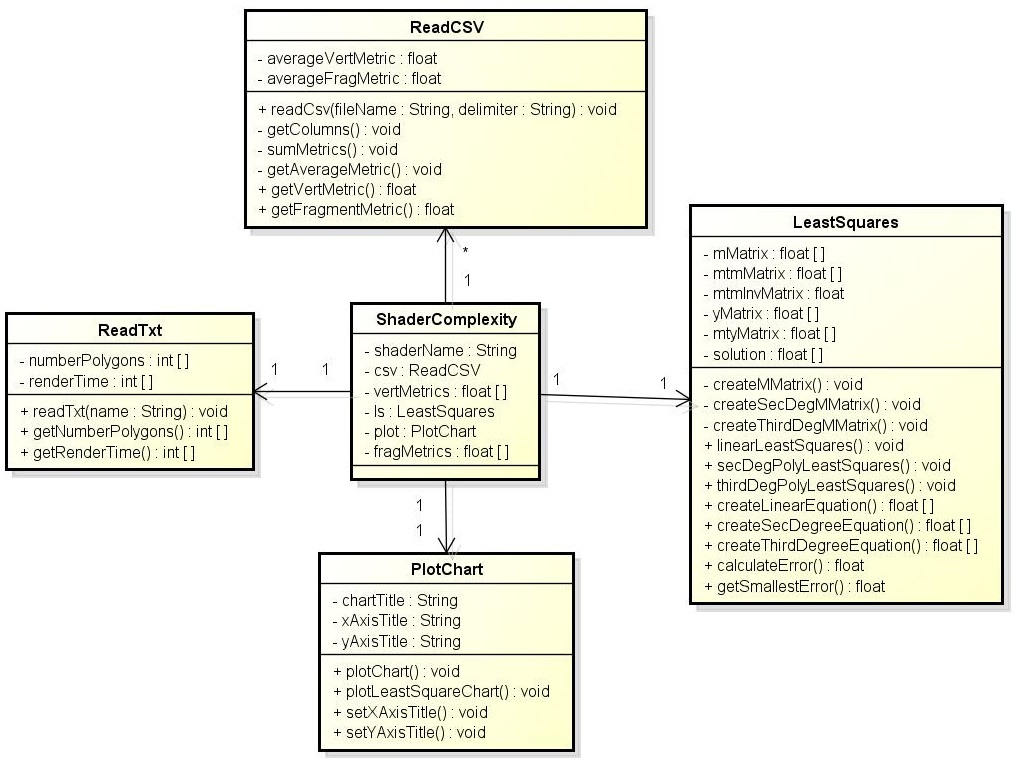
\includegraphics[keepaspectratio=true,scale=0.6]{figuras/minquad_diag.jpg}
	\caption{Diagrama de Classes do código de automatização}
	\label{minquad_diag}
	\end{figure}


\section{Análise Numérica}


	Para cada \textit{shader} foram plotados os gráficos para a métrica de vértice e para a de fragmento. Após as plotagens, percebeu-se que todos os gráficos de todos os \textit{shaders} relacionados ao vértice deram uma função linear (diferindo na inclinação), e os relacionados ao fragmento deram uma curva semelhante (como pode ser visto na Figura \ref{plotred} e na Figura \ref{plotrefl}). A primeira são os gráficos relacionados ao \textit{ red shader} (mais simples) e o segundo ao \textit{reflection shader} (mais complexo). 

	\begin{figure}[h]
	\centering
		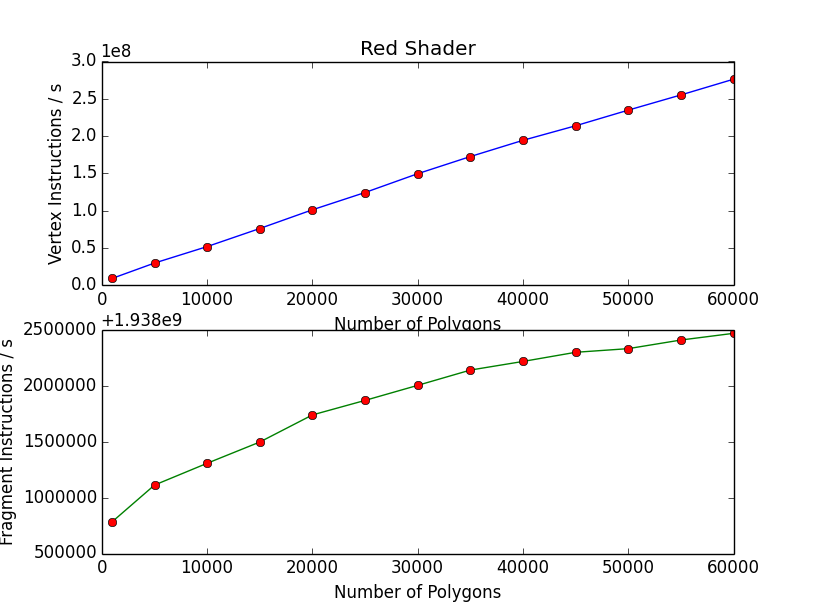
\includegraphics[keepaspectratio=true,scale=0.6]{figuras/red.png}
	\caption{Gráficos: \textit{red shader}}
	\label{plotred}
	\end{figure}

	\begin{figure}[h]
	\centering
		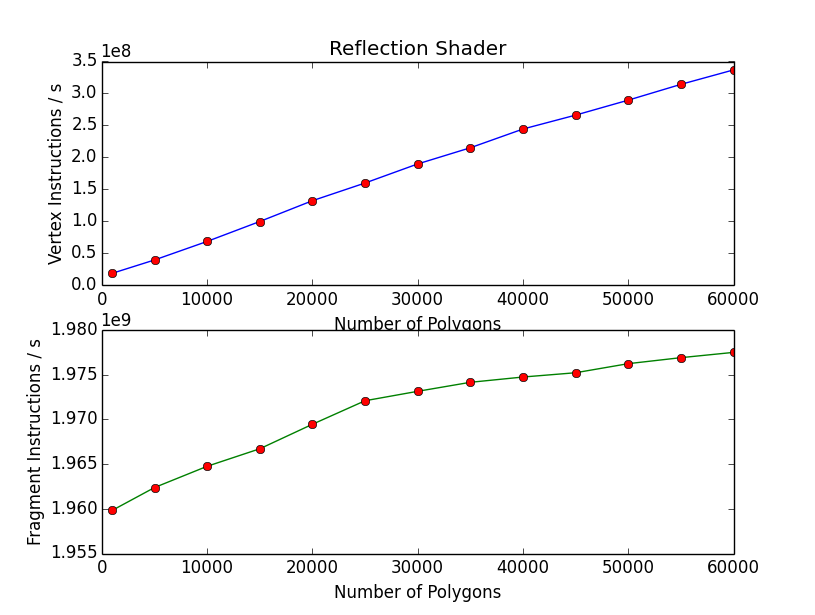
\includegraphics[keepaspectratio=true,scale=0.6]{figuras/reflectionplot.png}
	\caption{Gráficos: \textit{reflection shader}}
	\label{plotrefl}
	\end{figure}	


	 Os ajustes de cada curva (linear, exponencial, segundo e terceiro graus) também foram plotados (Figura \ref{linear}, Figura \ref{exp}, Figura \ref{sec} e Figura \ref{third}), em que avisa-se qual foi o menor erro associado. Pela a análise do menor erro, calculado de acordo com a Seção ADICIONAR SEÇÃO, todos os \textit{shaders} indicaram uma curva de segundo grau.

	\begin{figure}[h]
	\centering
		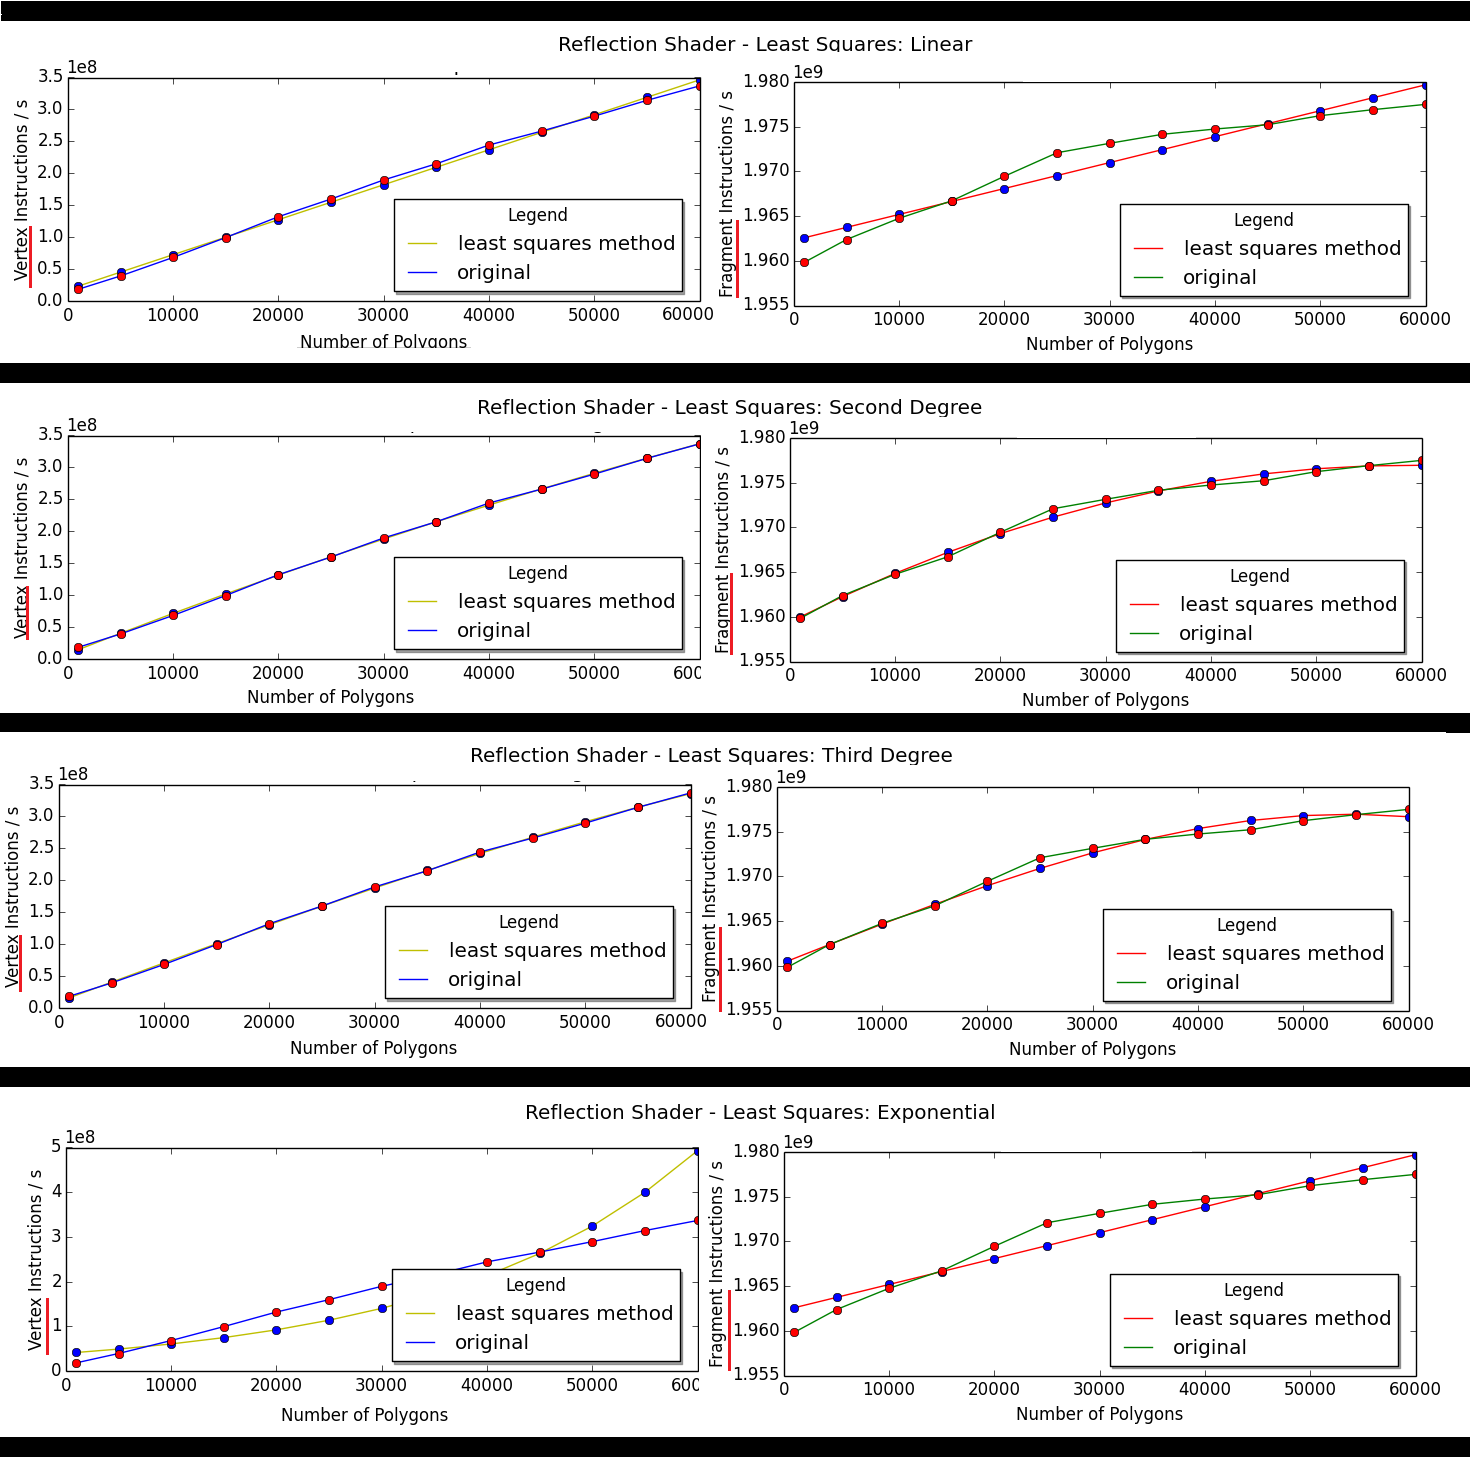
\includegraphics[keepaspectratio=true,scale=0.4]{figuras/reflectionlinear.png}
	\caption{Ajuste linear}
	\label{linear}
	\end{figure}	

	\begin{figure}[h]
	\centering
		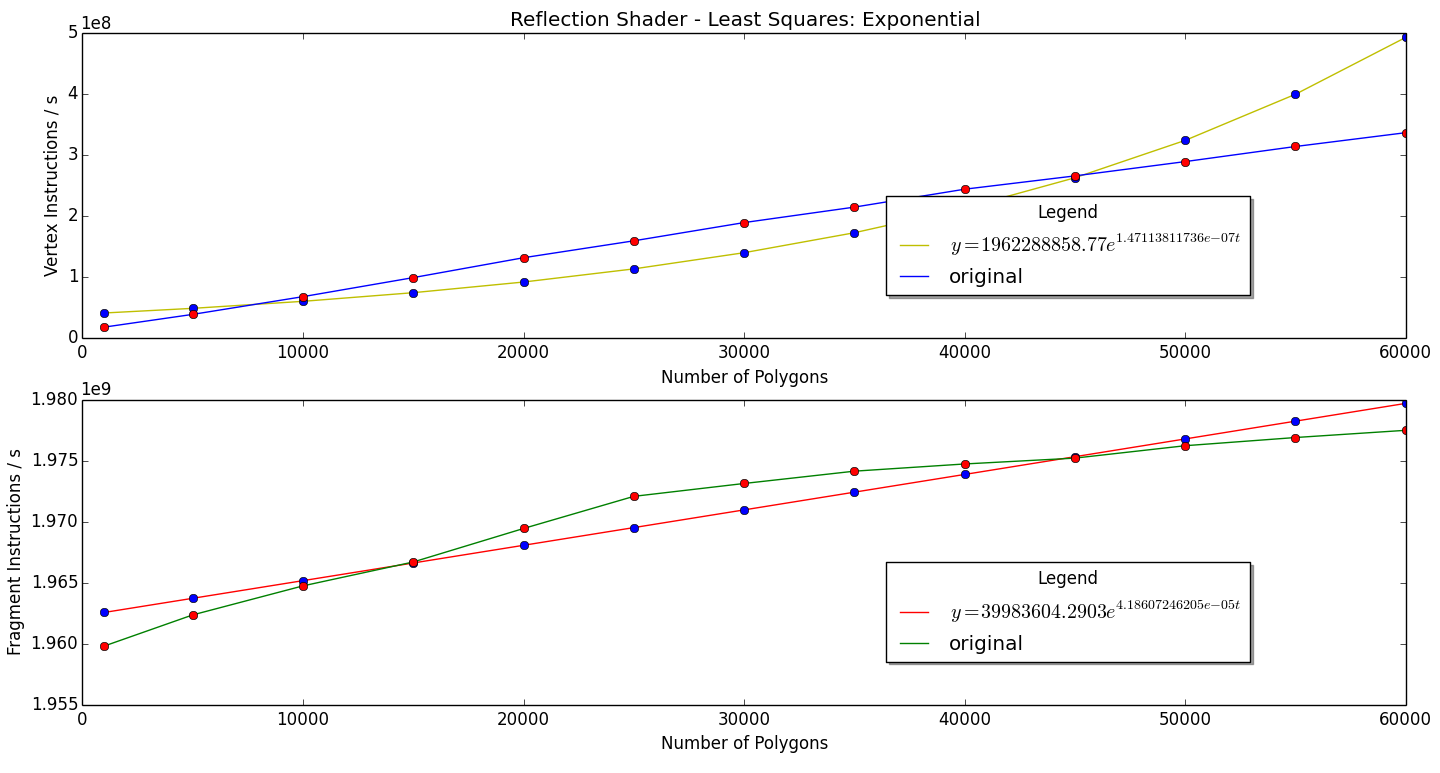
\includegraphics[keepaspectratio=true,scale=0.4]{figuras/reflectionexponential.png}
	\caption{Ajuste exponencial}
	\label{exp}
	\end{figure}	

	\begin{figure}[h]
	\centering
		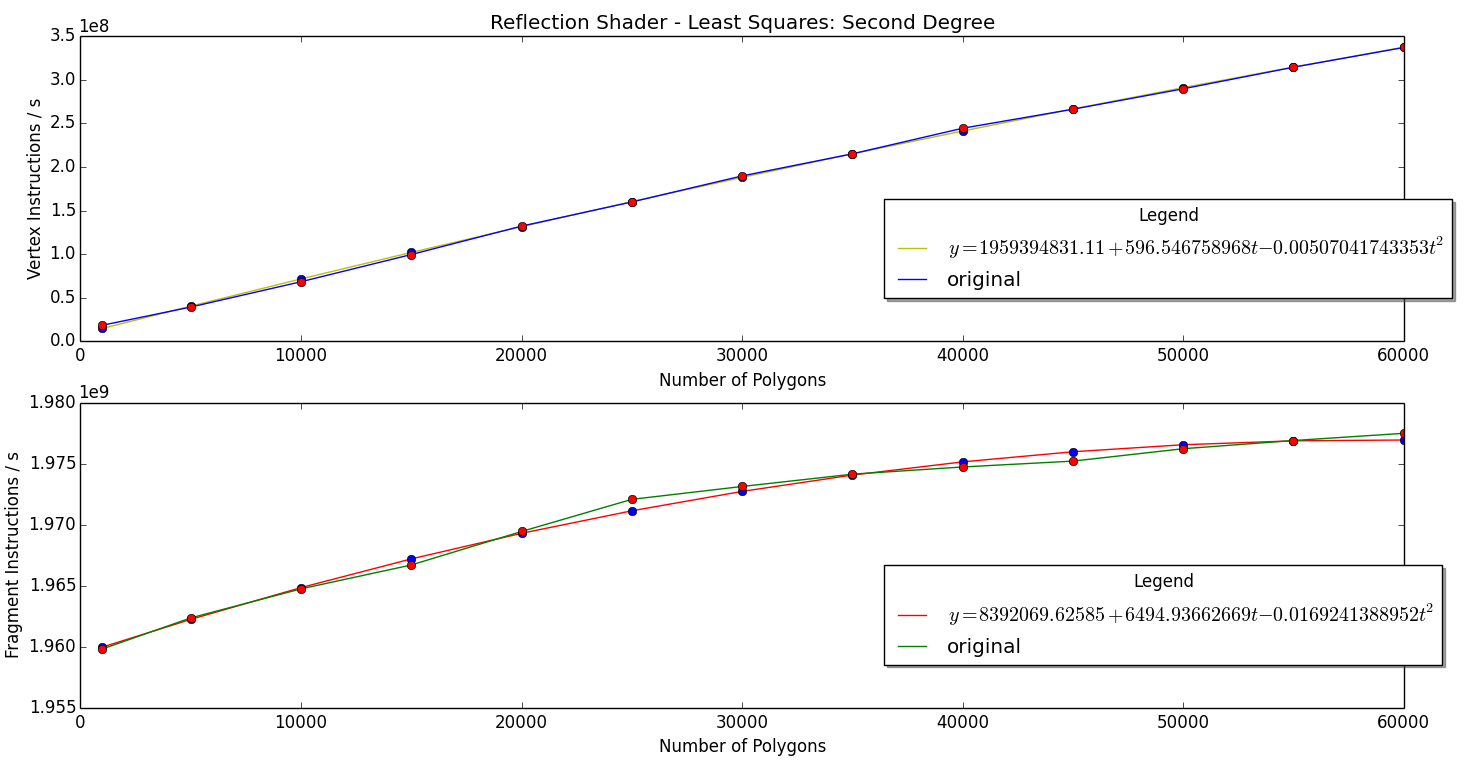
\includegraphics[keepaspectratio=true,scale=0.4]{figuras/reflectionsec.png}
	\caption{Ajuste função de segundo grau}
	\label{sec}
	\end{figure}	

	\begin{figure}[h]
	\centering
		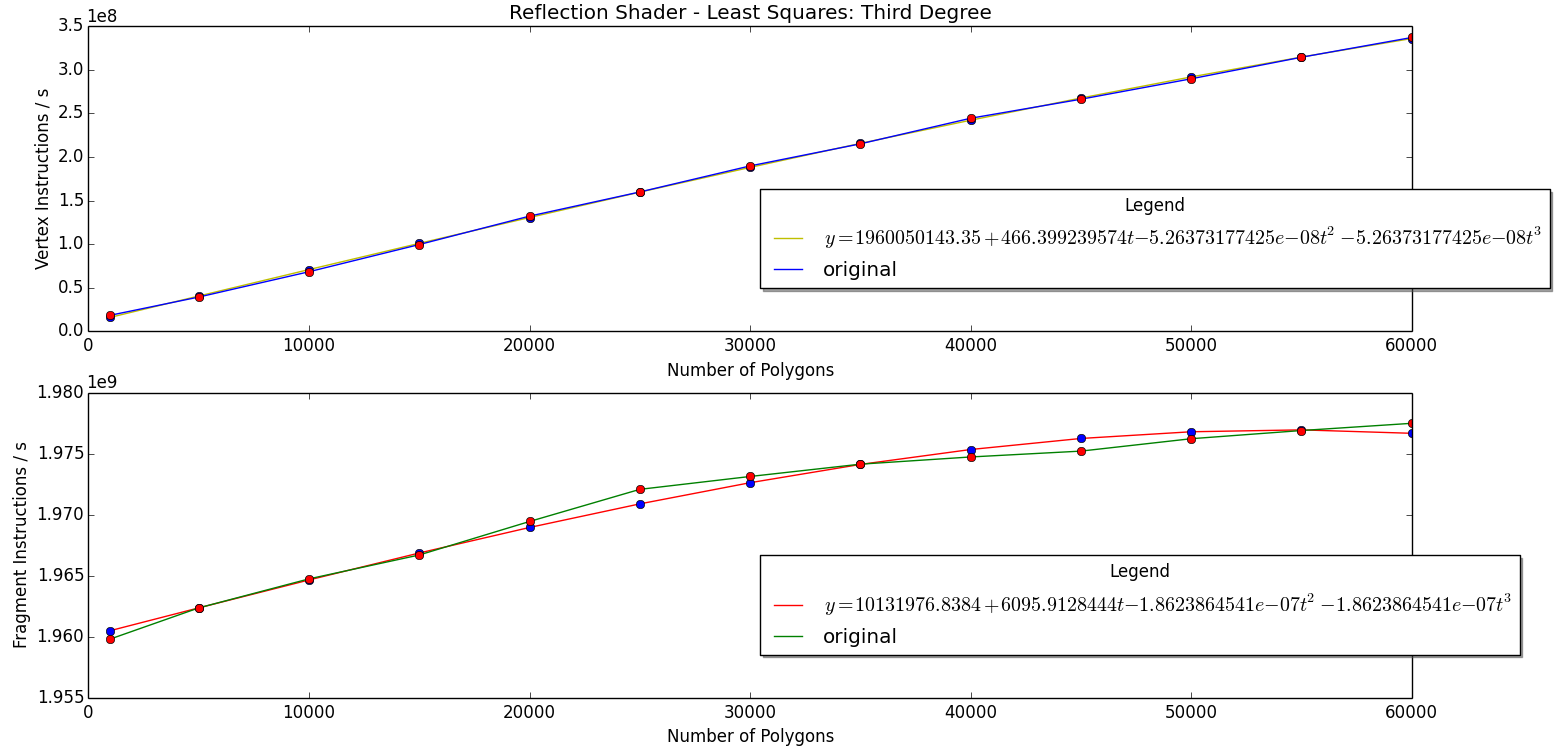
\includegraphics[keepaspectratio=true,scale=0.4]{figuras/reflectionthird.png}
	\caption{Ajuste função de terceiro grau}
	\label{third}
	\end{figure}	

	As equações calculadas para cada \textit{shader} (relacionadas ao vértice e fragmento) são mostradas na Tabela \ref{equacoes}.


	\begin{table}[h]
	\centering	
	\begin{tabularx}{0.9\textwidth}{cXX}
		\toprule
		\textbf{Nome} & \textbf{\textit{Equação Vertex Shader}} & \textbf{\textit{Equação Fragment Shader}}  \\
		\midrule
		\textit{Gouraud} & $y = 19.92 x 10^8 + 509.43t$ & $y = 67.99 x 10 ^5 + 6076.30t - 0.014t^2$ \\
		\textit{Phong} &  $y = 19.45 x 10^8 + 74.85t$ & $y = 20.20 x 10^6 + 9605.32t - 0.035t^2$\\
		\textit{Red} & $y = 19.39 x 10^8 + 26.84t$ & $y = 29.95 x 10 ^5 + 5130.50t - 0.0097t^2$ \\
		\textit{Toon} & $y = 19.45 x 10^8 + 100.35t$ & $y = 38.25 x 10 ^5 + 5347.86t - 0.011t^2$ \\
		\textit{Flat} & $y = 19.39 x 10^8 + 26.77t$ & $y = 25.02 x 10 ^5 + 4285.80t - 0.0091t^2$ \\
		\textit{Random Color} & $y = 19.45 x 10^8 + 74.04t$ & $y = 84.32 x 10 ^5 + 6930.50t - 0.021t^2$ \\
		\textit{Simple Texture} & $y = 19.42 x 10^8 + 49.97t$ & $y = 31.76 x 10 ^5 + 5137.26t - 0.0099t^2$ \\
		\textit{CubeMap} & $y = 19.44 x 10^8 + 83.38t$ & $y = 33.14 x 10 ^5 + 5109.61t - 0.0094t^2$ \\
		\textit{Reflection} & $y = 19.62 x 10^8 + 289.76t$ & $y = 83.92 x 10 ^5 + 6494.94t - 0.017t^2$ \\
	
		\bottomrule
	\end{tabularx}
	\caption{Equações relacionadas ao \textit{vertex shader} e \textit{fragment shader}}
	\label{equacoes}
	\end{table}
